% Created 2020-05-08 Fri 15:50
% Intended LaTeX compiler: pdflatex
\documentclass[12pt]{report}
\usepackage[utf8]{inputenc}
\usepackage[T1]{fontenc}
\usepackage{graphicx}
\usepackage{grffile}
\usepackage{longtable}
\usepackage{wrapfig}
\usepackage{rotating}
\usepackage[normalem]{ulem}
\usepackage{amsmath}
\usepackage{textcomp}
\usepackage{amssymb}
\usepackage{capt-of}
\usepackage{hyperref}
\setlength{\parindent}{0pt}
\usepackage[margin=1in]{geometry}
\usepackage{emptypage}
\usepackage{tikz}
\usetikzlibrary{graphs,graphs.standard,bayesnet,arrows.meta,shapes.arrows}

% Colorlinks sets pdfborder to zero.
%\hypersetup{colorlinks,linkcolor=,urlcolor=gray}

%\usepackage[a4paper,top=2.25cm,bottom=2.25cm,left=3.0cm,right=3.0cm]{geometry}

%% arial font?????????
%% \usepackage[scaled]{uarial}
%% \renewcommand*\familydefault{\sfdefault} %% Only if the base font of the document is to be sans serif
%% \usepackage[T1]{fontenc}

\makeatletter
\renewenvironment{abstract}{%
    \if@twocolumn
      \section*{\abstractname}%
    \else %% <- here I've removed \small
      \begin{center}%
        {\bfseries \Huge\abstractname\vspace{\z@}}%  %% <- here I've added \Large
      \end{center}%
      \quotation
    \fi}
    {\if@twocolumn\else\endquotation\fi}
\makeatother

%\pagecolor{yellow!10}

\documentclass{book}
\usepackage{sectsty}
\chapternumberfont{\large} 
\chaptertitlefont{\huge}

\usepackage{hyperref}
\hypersetup{%
  colorlinks=false,% hyperlinks will be black
  linkbordercolor=red,% hyperlink borders will be red
  pdfborderstyle={/S/U/W 1}% border style will be underline of width 1pt
}

%% \usepackage[T1]{fontenc}
%% \usepackage{libertine}
%% \usepackage{graphicx}
%% \usepackage[svgnames]{xcolor}
%% \usepackage{framed}

%% \newcommand*\openquote{\makebox(25,-22){\scalebox{5}{``}}}
%% \newcommand*\closequote{\makebox(25,-22){\scalebox{5}{''}}}
%% \colorlet{shadecolor}{Azure}

%% \makeatletter
%% \newif\if@right
%% \def\shadequote{\@righttrue\shadequote@i}
%% \def\shadequote@i{\begin{snugshade}\begin{quote}\openquote}
%% \def\endshadequote{%
%%   \if@right\hfill\fi\closequote\end{quote}\end{snugshade}}
%% \@namedef{shadequote*}{\@rightfalse\shadequote@i}
%% \@namedef{endshadequote*}{\endshadequote}
%% \makeatother
%% \begin{document}


\author{Louis James}
\date{\today}
\title{Describing systems for exploring tangible and spatial computer interaction}
\hypersetup{
 pdfauthor={Louis James},
 pdftitle={Describing systems for exploring tangible and spatial computer interaction},
 pdfkeywords={},
 pdfsubject={Final year project for Creative Computing},
 pdfcreator={Emacs 26.3 (Org mode 9.3.6)}, 
 pdflang={English}}
\begin{document}

\maketitle

\renewcommand{\abstractname}{Acknowledgements}
\begin{abstract}
 Thanks to my family, Florent, Chudleigh dwellers, Jamie ...
\end{abstract}
\newpage


\renewcommand{\abstractname}{Abstract}
\begin{abstract}
Presented here is a specification of experimental approaches to computer
interaction based on spatial and tangible methods. The report describes an
prototypical implementation of a base system for interaction in space and a
theoretical API for such a system and similar systems. This utilises computer
vision techniques to analyse a surface to track objects and project onto the
space creating a feedback system for interaction. To finish a
ethnomethodological framework for evaluation and further development is
proposed???


\end{abstract}
\tableofcontents
\listoffigures
\chapter{Introduction}
\label{sec:org0965954}

\section{Project aims}
\label{sec:orgf1598c6}

\begin{itemize}
\item open source project for tangible interaction
\item Prototypical
\item ethnomethodological frameworks for evaluation
\end{itemize}

\chapter{Background}
\label{sec:orgc0202dc}

The motivation for this project stems in part from a feeling of frustration in
 how working on computers can often be a constricted affair and a pondering over
 how we might expand the \emph{keyboard-mouse-monitor} model to improve the utility
 of computers regarding our own perceptive abilities. How might a spatial,
 haptic and tangible environment for interaction create an improved space for
 working and thinking with computers as well with our physical health? How might
 such an environment fundamentally augment our cognitive capabilities; memory
 and learning as well as creativity itself?

\section{Definitions}
\label{sec:orgeb40a5c}
\begin{enumerate}
\item Computing
\label{sec:orga728bf0}
\item keyboard-mouse-monitor model (kmm model) (?)
\label{sec:org367d81e}
\item Cognition
\label{sec:orgb312ef3}
\item Exocortex
\label{sec:org43507c9}
\end{enumerate}

\section{Beginning with the Exocortex}
\label{sec:org956a0ea}

I started off looking at \emph{Exocortexes} and other personal archiving systems.
Systems that allow the user to externalise thought and memory. This could be via
simply storing and organising work and ideas efficiently and methodically or
unifying many tasks or different workflows into a singular interface. \\

Org mode is a good example of such a system. Org mode is a "computing
environment for authoring mixed natural and computer language documents"
\cite{Schulte:Davison:Dye:Dominik:2011:JSSOBK:v46i03}. It is designed for taking
notes, producing documents and organising and runs inside of the text editor,
Emacs. It has the ability to export to different formats such as HTML, \LaTeX{} and
supports "outlining, note-taking, hyperlinks, spreadsheets, TODO lists, project
planning, GTD" as well as literate programming, all in plain-text
\cite{Schulte:Davison:Dye:Dominik:2011:JSSOBK:v46i03}. (it is incidentally what
this document is produced with) \\


Another point of reference when I was looking at externalised 'artificial
information-processing systems' was Devine Lu Linvega's Exocortex \href{https://wiki.xxiivv.com/site/nataniev.html}{XXIIV --
nataniev}. \emph{XXIIV} is a personal archive and log with documentation of Linvega's
personal tools and artworks. The site has gone through some changes since I
first came across it. Originally a static, javascript and lisp based website
with diaries, blog type posts and categorised personal logs. It is now somewhat
stripped back in style and has been rewritten in \href{https://en.wikipedia.org/wiki/C99}{C (C99)}. The work contains a
selection of esoteric programming tools including a synthetic language, games,
software all logged using their own \emph{Arvelie calendar} \cite{DevineNataniev}. \\

Both these two systems have their own specific use-cases, \emph{Org-mode}; in
academia and science and \emph{XXIIV}; an experimental personal archive. They both
utilise the contemporary and prevailing \emph{keyboard-mouse-monitor} paradigm
of computer interaction but push the boundaries of cognition in this medium,
particularly regarding memory and productivity. These two projects were a birth
point in thinking about how software systems can be augment thought and improve
learning ability and computer productivity.


\section{A virtual exploration of Dynamicland}
\label{sec:orgc614bd2}

Another original and critical point of reference was \emph{Dynamicland}, a research
project in Oakland, USA. The aim of the project is to implement a new more
powerful and accessible model of computing.

\begin{quote}


In Oakland, we built the first full-scale realization of the vision, inviting
thousands of people into our space to collaborate. Together, these artists,
scientists, teachers, students, programmers, and non-programmers created
hundreds of projects that would have been impossible anywhere else.
-- Dynamicland.org 
\end{quote}


\emph{Dynamicland} is a communal computer where the building is the computer (ENIAC).
Programs are embodied in the room on pieces of colour-coded paper. The programs
are recognised via the codes and their code, stored in a database is then run,
it can also \emph{read} code using OCR but generally the code is there \href{https://thenewstack.io/dynamicland-rethinks-computer-interfaces/}{symbolically}.
Projectors on the ceiling transform the paper and workbenches into whatever the
programmer decides. This relatively simple model makes for an exciting new
ecosystem for collaborative computing and expressive programming. Victors,
highlights his ideas for the progression of computing and interaction in a
series of talks (available online) and on his \href{http://worrydream.com}{website}. In his talk "Seeing
Spaces" he talks of a new kind of maker-space which allow makers to see across
time and possibilities. \emph{Dynamicland} offers a computational medium which allows
for full use of the human senses and a more \href{https://vimeo.com/115154289}{humane representation of thought}
\cite{VictorKayDynamicLand}. \\

\begin{figure}[htbp]
\centering
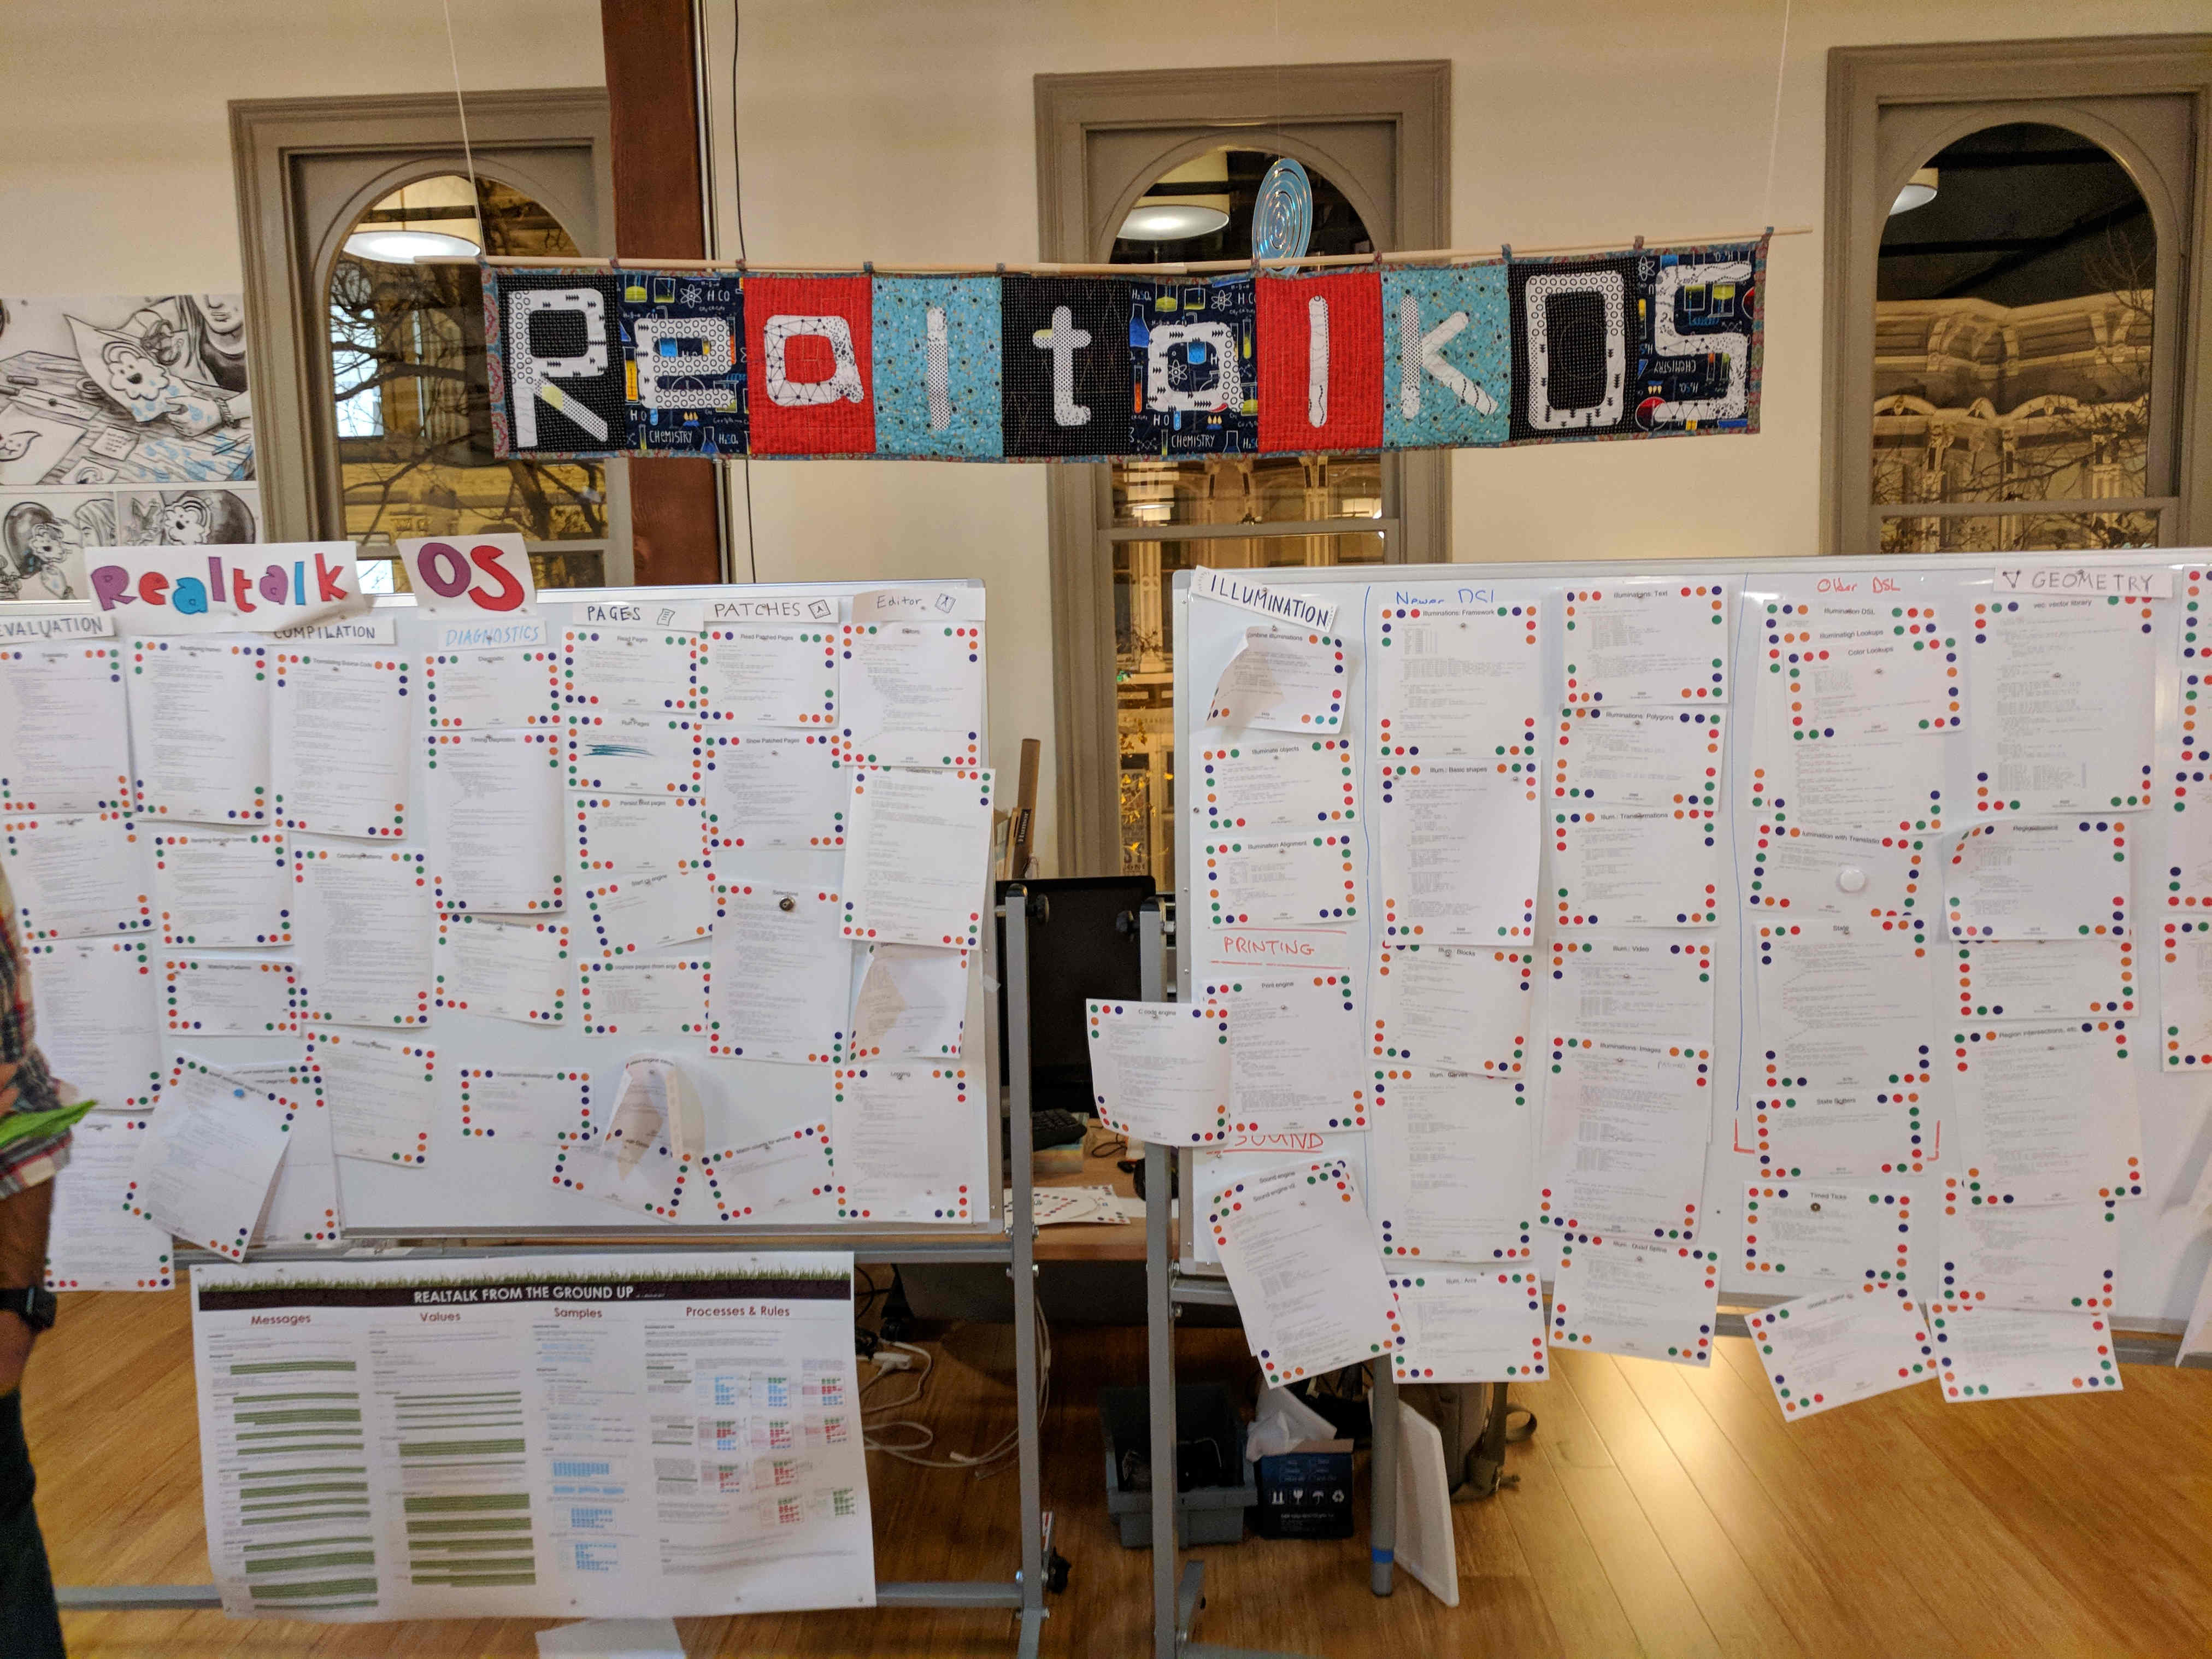
\includegraphics[width=12cm]{assets/realtalk-os.jpg}
\caption{RealtalkOS, the operating system of \emph{Dynamicland}}
\end{figure}  


\emph{DL} was the inspiration for the main physical and technical model for
this project, an \emph{augmented} workspace either on the floor or a table which is
projected onto. A camera/s pointing down onto the projection space is the sensor
for detecting interaction, with the projector as the actuator. This base model can be
seen in Figures \ref{pp-schema} and  \ref{systemSchema}.

\section{Paper programs - open source}
\label{sec:org905e499}

Looking to find some of the code for \emph{Dynamicland} and a more detailed
specification of \textbf{DL} I stumbled across \emph{Paper Programs} (\emph{Dynamicland} has an
'open-source model', but it is only open if you can visit it physically as the
source code is physically in the space). \emph{Paper Programs} is a browser-based
partial clone of \emph{Dynamicland}. This was another starting point for playing
around with but I found that I couldn't set it up and have it stable enough to
develop on. It also suffers from being quite slow, due to the Computer Vision
and graphics being done in the browser (it uses a version of OpenCv compiled to
\href{https://webassembly.org/}{WebAssembly}) \cite{JpPaperPrograms}.


\section{Sage digital research}
\label{sec:orgfa568bc}

Ethnomethodology

Embodied Cognition

Haptic interfaces

\section{MIT Prof - tangible media group}
\label{sec:orga3e112a}
\url{http://tangible.media.mit.edu/projects/}
\section{Nielsen: augmenting ltm and using ai to augment human-i ??????}
\label{sec:orgf0ca617}

Other approaches to 

\cite{NielsenMich2018altm}

\cite{carter2017using}  

\section{Tangible bits - Hiroshi Ishii  and  Brygg Ullmer}
\label{sec:orgee569e3}
\cite{IshiiH2002Tbdt}

\chapter{Specification and context}
\label{sec:org6e7f0ef}

\begin{figure}[htbp]
\centering
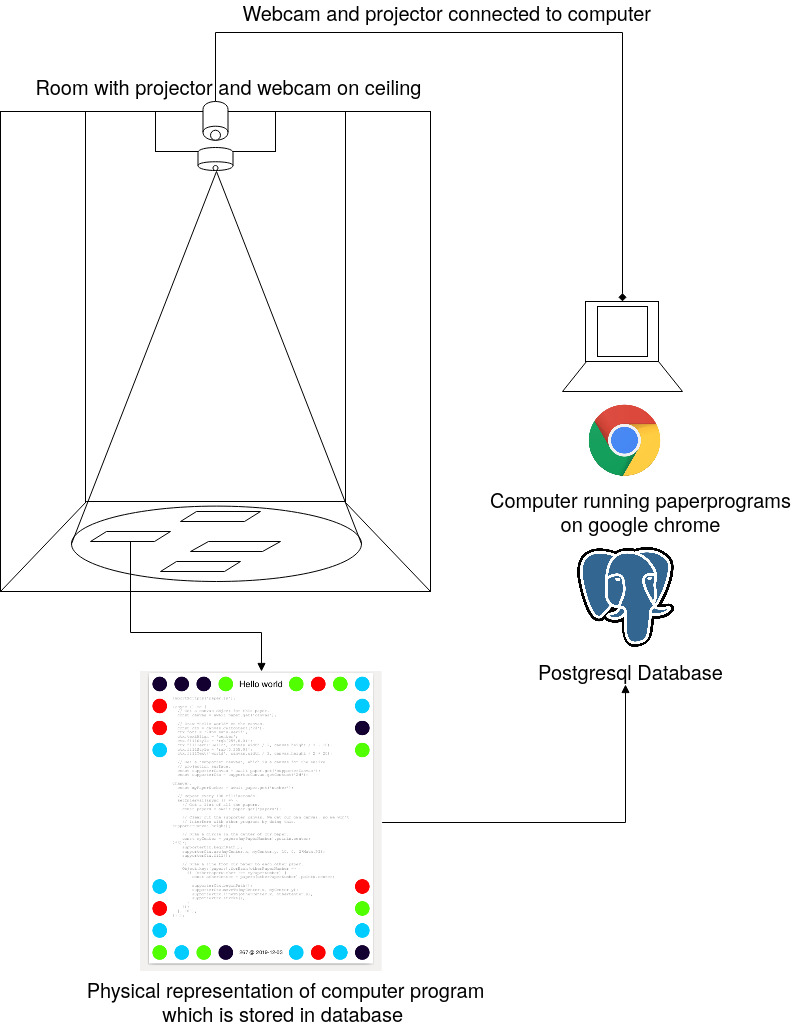
\includegraphics[width=15cm]{assets/pp-diag.png}
\caption{The initial physical schema: \emph{Paperprograms} \label{pp-schema}}
\end{figure}


\chapter{Project in depth}
\label{sec:orgaf198c3}

See system schema Fig.  

\begin{figure}[htbp]
\centering
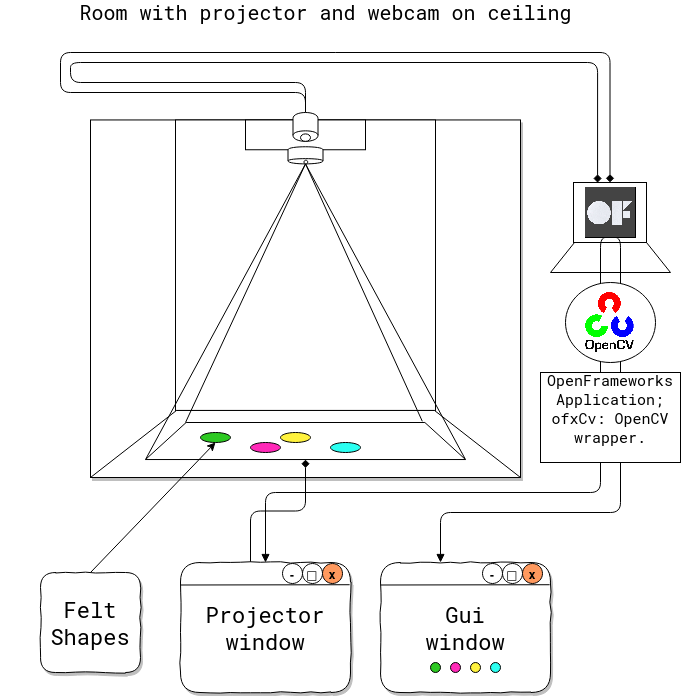
\includegraphics[width=15cm]{assets/project-schema-final.png}
\caption{System schema \label{systemSchema}}
\end{figure}


\chapter{Creative process}
\label{sec:orgeba3de9}
\chapter{Debugging and problem solving}
\label{sec:org04b6182}
\chapter{Evaluation and Conclusions}
\label{sec:orgb1ec848}
\bibliographystyle{ieeetr} 
\bibliography{references}
\end{document}
